\begin{table*}[t]
\centering
\caption{Effectiveness and efficiency comparison on \textsc{LongMemEval-S}. The token usage is in thousands. -- indicates no value for the metric. \textbf{Bold} denotes the best result, \underline{underline} the second-best. $r$ denotes the compression rate. $th$ denotes the capacity threshold of the STM buffer, measured in tokens. 
Each pair of $r$ and $th$ corresponds to two rows: one for online soft update and one for offline update. OP-update denotes the offline parallel update process of \textbf{LightMem}.
} 
\renewcommand{\arraystretch}{1.00}
\setlength{\tabcolsep}{2.5pt}
\setlength\dashlinedash{1.0pt}  % 点的长度
\setlength\dashlinegap{2pt}     % 间距
\small
\scalebox{1.00}{
\begin{tabular}{@{}lcccccccc@{}}
\toprule
\multirow{2}{*}{\textbf{Method}} & \multirow{2}{*}{\textbf{ACC (\%)}} & 
\multicolumn{2}{c}{\textbf{Summary Tokens (k)}} & 
\multicolumn{2}{c}{\textbf{Update Tokens (k)}} & 
\multirow{2}{*}{\textbf{Total (k)}} & 
\multirow{2}{*}{\textbf{Calls}} & 
\multirow{2}{*}{\textbf{Runtime (s)}} \\
\cmidrule(lr){3-4}\cmidrule(lr){5-6}
 &  & \textbf{In} & \textbf{Out} & \textbf{In} & \textbf{Out} &  &  &  \\
\midrule

% ===== GPT-4o-mini 分区 =====
\rowcolor{gptbar}\multicolumn{9}{c}{\openailogo\ \textbf{GPT-4o-mini}}\\
\midrule
\rowcolor{gptgray} FullText          & 56.80 & --      & --     & --  & --  & 105.07 & --  & -- \\
\rowcolor{gptgray} NaiveRAG          & 61.00 & --      & --     & --  & --  & -- & --  & 867.38 \\
\rowcolor{gptgray} LangMem          & 37.20 & --      & --     & 982.68  & 119.48  & 1,102.16 & 520.62  & 2,293.70 \\
\rowcolor{gptgray} A-MEM            & 62.60 & 214.66  & 42.82  & 1,157.52& 190.81  & 1,605.81 & 986.55 & 5,132.06 \\
\rowcolor{gptgray} MemoryOS         & 44.80 & 2,302.35& 304.18 & 350.02  & 35.19   & 2,991.75 & 2,938.41& 8,030.04 \\
\rowcolor{gptgray} Mem0             & 53.61 & 424.13  & 17.76  & 560.17  & 150.56  & 1,152.62 & 811.57  & 4,248.49 \\
\hdashline
\rowcolor{gptgray} 
LightMem                  & & & & & & & &\\
\rowcolor{gptgray}
$r$=0.5, $th$=256 & 64.29 & \underline{20.80} & \underline{10.01} & -- & -- & \underline{30.81} & \underline{25.67} & \underline{302.69} \\
\rowcolor{gptgray} (OP-update) & 64.69 & -- & -- & \textbf{44.46} & \textbf{2.56} & 47.02 & 70.23 & 342.63 \\
\rowcolor{gptgray} 
$r$=0.6, $th$=256 & \underline{67.78} & 24.58 & 10.53 & -- & -- & 35.11 & 30.47 & 329.61 \\
\rowcolor{gptgray} (OP-update) & 65.39 & -- & -- & \underline{53.98} & \underline{3.18} & 57.16 & 85.07 & 411.56 \\
\rowcolor{gptgray} 
 $r$=0.7, $th$=512 & \textbf{68.64} & \textbf{18.88} & \textbf{9.37} & -- & -- & \textbf{28.25} & \textbf{18.43} & \textbf{283.76} \\
 \rowcolor{gptgray} (OP-update) & 67.07 & -- & -- & 79.38 & 4.06 & 83.44 & 125.47 & 496.03 \\

\addlinespace[0.4ex]
\midrule

% ===== Qwen 分区 =====
\rowcolor{qwenbar}\multicolumn{9}{c}{\qwenlogo\ \textbf{Qwen3-30B-A3B-Instruct-2507}}\\
\midrule
\rowcolor{qwenlav} FullText          & 54.80    & --      & --     & --      & --      & 105.07       & --       & -- \\
\rowcolor{qwenlav} NaiveRAG          & 60.80    & --      & --     & --      & --      & --       & --       & 659.09 \\
\rowcolor{qwenlav} LangMem          & 50.80    & --      & --     & 1,311.96      & 118.06      & 1,430.02       & 495.12       & 3,237.16 \\
\rowcolor{qwenlav} A-MEM            & 65.20    & 219.21      & 66.98     & 1,260.54      & 318.20      & 1,864.93       & 989.30     & 5,367.51 \\
\rowcolor{qwenlav} MemoryOS         & 49.60 & 2,101.54& 510.88 & 305.12  & 27.43   & 2,944.97 & 2,922.28 & 8,721.78 \\
\rowcolor{qwenlav} Mem0             & 39.51 & 424.20 & \textbf{15.34}  & 411.50  & 111.35  &  1001.90  & 722.76 & 2,239.94 \\

\hdashline

\rowcolor{qwenlav} 
LightMem                  & & & & & & & &\\
\rowcolor{qwenlav} 
$r$=0.4, $th$=768 & 61.95 & \textbf{9.01} & \underline{16.14} & -- & -- & \textbf{25.15} & \underline{16.54} & \underline{357.13} \\
\rowcolor{qwenlav} 
(OP-update) & 62.34 & -- & -- & 111.13 & 7.88 & 119.01 & 176.02 & 1036.47 \\
\rowcolor{qwenlav} 
$r$=0.6, $th$=768 & \textbf{70.20} & \underline{13.19} & 19.21 & -- & -- & \underline{32.40} & 19.97 & 417.13 \\
\rowcolor{qwenlav} 
(OP-update) & 65.14 & -- & -- & \textbf{97.11} & \textbf{5.92} & 103.03 & 152.93 & 1023.56 \\
\rowcolor{qwenlav} 
$r$=0.8, $th$=1024 & \underline{68.69} & 14.82 & 18.49 & -- & -- & 33.31 & \textbf{9.43} & \textbf{355.71} \\
\rowcolor{qwenlav} 
(OP-update) & 67.34 & -- & -- & \underline{106.91} & \underline{6.20} & 113.11 & 168.37 & 1026.90 \\

\addlinespace[0.4ex]
\midrule

% ===== GLM 分区 =====
\rowcolor{glmblue}\multicolumn{9}{c}{\zhipulogo\ \textbf{GLM-4.6}}\\
\midrule
\rowcolor{glmblue} FullText          & 36.71 & --      & --      & --      & --      & 103.38 & --     & -- \\
\rowcolor{glmblue} NaiveRAG          & \textbf{73.20} & --      & --      & --      & --      & --     & --     & 53,725.15 \\
\rowcolor{glmblue} LangMem           & 49.20 & --      & --      & 3,052.42 & 7.03   & 3,059.45 & 314.61 & 5,577.91 \\
\rowcolor{glmblue} A-MEM             & 70.60 & 444.95  & 63.40   & 1,992.04 & 403.39 & 2,903.78 & 450.40 & 8,068.80 \\
\hdashline
\rowcolor{glmblue} LightMem           &       &         &         &         &         &         &        &        \\
\rowcolor{glmblue} 
$r$=0.5, $th$=256 & \underline{73.00} & \underline{16.55} & 14.06 & -- & -- & \underline{30.61} & \underline{10.78} & \textbf{1,014.37} \\
\rowcolor{glmblue} 
$r$=0.6, $th$=256 & \textbf{73.20} & \textbf{16.55} & \underline{13.99} & -- & -- & 30.54 & \textbf{10.78} & 1,077.69 \\
\rowcolor{glmblue} 
$r$=0.7, $th$=512 & 72.80 & \textbf{16.55} & \textbf{13.91} & -- & -- & \textbf{30.46} & 10.78 & \underline{1,038.19} \\

\bottomrule
\end{tabular}}
\label{tab:memory_comparison}
\end{table*}


\section{experiments}

\subsection{experimental setup}
\noindent \textbf{Experimental Details.}
(1) Our experiments adopt a realistic \textbf{\textit{Incremental Dialogue Turn Feeding}} setting, where the entire dialogue history is fed and processed \textbf{at the turn level, one turn at a time}. 
This reflects practical scenarios where interactions between user and model is incrementally formed turn by turn.~\citep{hu2025evaluatingmemoryllmagents}.
(2) For considerations of both efficiency and effectiveness, we employ LLMLingua-2 as our pre-compressor throughout all subsequent experiments. 
(3) The attention scores for topic segmentation are also obtained using LLMLingua-2, the size of the sensory memory buffer is 512 tokens. 
All specific models used in this paper, can be found in Table~\ref{tab:function_model_map}. 

\noindent \textbf{Datasets \& Baseline Methods.}
\change{We use two well-known datasets, \textsc{LongMemEval}~\citep{DBLP:conf/iclr/WuWYZCY25} (specifically the LongMemEval-S split) and \textsc{LoCoMo}~\citep{maharana2024evaluatinglongtermconversationalmemory} to evaluate memory ability.}
We compare \textbf{LightMem} against several representative baselines of conversational memory modeling. 
\ding{172} \textit{Full Text}, 
\ding{173} \textit{Naive RAG}, 
\ding{174} \textit{LangMem}~\citep{LangMemBlog},
\ding{175} \textit{A-MEM}~\citep{Xu2025AMEMAM}, 
\ding{176} \textit{MemoryOS}~\citep{Kang2025MemoryOO}, 
\ding{177} \textit{Mem0}~\citep{Chhikara2025Mem0BP}. 
In addition, all methods use GPT-4o-mini, Qwen3-30B-A3B-Instruct-2507 and GLM-4.6 as the LLM backbones.
Details on dataset, baselines, and experimental settings are provided in the Appendix~\ref{experiment_detail}. 

\noindent \textbf{Metrics.}
We evaluate these methods using both effectiveness and efficiency metrics. 
For effectiveness, we report \textbf{Accuracy (ACC)}, defined as the proportion of correctly answered questions. 
The evaluation is conducted with \emph{GPT-4o-mini} as an LLM judge, guided by a detailed evaluation prompt (see Appendix~\ref{prompts:LLM-as-Judge}). 
For efficiency, we focus on tracking the computational costs of the LLM invocations in memory bank construction stage (see Section~\ref{main_text_preliminary}), all averaged across the entire dataset, as it is the one tied to the design and implementation differences of memory systems. 
The retrieval and usage stage is not our focus, because for fair comparison, The $f_{\text{retrieve}}()$, $f_{\text{chat}}()$ and number of retrieved entries are same among all methods. As a result, their costs exhibit only minor differences, and this stage is largely orthogonal to the design of memory systems, as shown in the table. 
Within the memory bank construction stage, only the two sub-processes  \textbf{Summary} and \textbf{Update} involve the use of LLMs, $f_{\text{sum/extract}}()$ and $f_{\text{update}}()$. 
So for both processes, we report the token consumption from LLM calls, including input tokens, output tokens, and total token usage (in thousands). 
Additionally, we track \textbf{API Calls} counting the total number of LLM invocations, and \textbf{Runtime} recording the overall execution time for memory bank construction stage. 
% as indicated in Table~\ref{tab:rag_cost_time}, 

\begin{table*}[t]
\centering
\caption{\change{Effectiveness and efficiency comparison on \textsc{LoCoMo}. Due to space limitations and for ease of comparison, we merge the results before and after LightMem’s offline update into a single row. The ACC reported corresponds to the performance after the offline update.
}}
\renewcommand{\arraystretch}{1.00}
\setlength{\tabcolsep}{2.5pt}
\setlength\dashlinedash{1.0pt}
\setlength\dashlinegap{2pt}
\small
\scalebox{1.00}{
\begin{tabular}{@{}lcccccccc@{}}
\toprule
\multirow{2}{*}{\textbf{Method}} & \multirow{2}{*}{\textbf{ACC (\%)}} & 
\multicolumn{2}{c}{\textbf{Summary Tokens (k)}} & 
\multicolumn{2}{c}{\textbf{Update Tokens (k)}} & 
\multirow{2}{*}{\textbf{Total (k)}} & 
\multirow{2}{*}{\textbf{Calls}} & 
\multirow{2}{*}{\textbf{Runtime (s)}} \\
\cmidrule(lr){3-4}\cmidrule(lr){5-6}
 &  & \textbf{In} & \textbf{Out} & \textbf{In} & \textbf{Out} &  &  &  \\
\midrule

% ===== GPT-4o-mini 分区 =====
\rowcolor{gptbar}\multicolumn{9}{c}{\openailogo\ \textbf{GPT-4o-mini}}\\
\midrule
\rowcolor{gptgray} FullText          & 71.83 & -- & -- & -- & -- & -- & -- & -- \\
\rowcolor{gptgray} NaiveRAG          & 63.64 & -- & -- & -- & -- & -- & -- & -- \\
\rowcolor{gptgray} LangMem           & 57.20 & -- & -- & 898.27 & 111.95 & 1010.22 & 920.62 & 2229.37 \\
\rowcolor{gptgray} A-MEM             & 64.16 & 182.74 & 49.29 & 729.89 & 187.52 & 1149.43 & 1175.47 & 6060.73 \\
\rowcolor{gptgray} MemoryOS(locomo)\footnotemark   & 58.25 & 110.98 & 33.40 & 78.08  & 64.54 & 287.00 & 553.45 & 2422.05 \\
\rowcolor{gptgray} MemoryOS(regular)  & 54.87 & 226.86 & 46.61 & 177.66 & 75.34 & 526.48 & 1016.06 & 3332.59 \\
\rowcolor{gptgray} Mem0              & 61.69 & 851.32 & 20.53 & 632.12 & 189.42 & 1693.39 & 1602.20 & 4432.87 \\
\hdashline
\rowcolor{gptgray} LightMem(0.7,512) & \underline{71.95} & 73.19 & 20.13 & 6.05 & 0.40 & 99.76 & 41.65 & 848.49 \\
\rowcolor{gptgray} LightMem(0.7,768) & 70.26 & \textbf{57.54} & \underline{18.92} & \textbf{3.79} & \textbf{0.23} & \textbf{80.48} & \textbf{29.55} & \textbf{737.80} \\
\rowcolor{gptgray} LightMem(0.8,768) & \textbf{72.99} & \underline{62.82} & \textbf{17.95} & \underline{4.14} & \underline{0.28} & \underline{85.19} & \underline{29.83} & \underline{815.32} \\

\addlinespace[0.4ex]
\midrule

% ===== Qwen 分区 =====
\rowcolor{qwenbar}\multicolumn{9}{c}{\qwenlogo\ \textbf{Qwen3-30B-A3B-Instruct-2507}}\\
\midrule
\rowcolor{qwenlav} FullText          & \textbf{74.87} & -- & -- & -- & -- & -- & -- & -- \\
\rowcolor{qwenlav} NaiveRAG          & 66.95 & -- & -- & -- & -- & -- & -- & -- \\
\rowcolor{qwenlav} LangMem           & 60.53 & -- & -- & 1004.35 & 138.02 & 1142.37 & 1005.37 & 2268.57 \\
\rowcolor{qwenlav} A-MEM             & 56.10 & 158.29 & 60.85 & 924.19 & 483.51 & 1626.80 & 1175.40 & 5543.90 \\
\rowcolor{qwenlav} MemoryOS(locomo)  & 61.04 & 122.21 & 53.12 & 104.43 & 81.75 & 361.51 & 414.70 & 1269.70 \\
\rowcolor{qwenlav} MemoryOS(regular)  & 51.30 & 228.85 & 51.60 & 242.27 & 143.63 & 666.35 & 1004.60 & 1982.20 \\
\rowcolor{qwenlav} Mem0              & 43.31 & 827.09 & \textbf{18.64} & 763.88 & 189.80 & 1799.40 & 1614.50 & 4540.70 \\
\hdashline
\rowcolor{qwenlav} LightMem(0.6,768)  & 71.36 & \textbf{56.68} & \underline{34.14} & \textbf{8.31} & \textbf{0.74} & \textbf{99.87} & \textbf{29.10} & \textbf{815.70} \\
\rowcolor{qwenlav} LightMem(0.8,1024) & \underline{72.60} & \underline{61.38} & 36.33 & \underline{9.86} & \underline{0.88} & \underline{108.45} & \underline{32.00} & \underline{1079.40} \\

% \addlinespace[0.4ex]
% \midrule

% % ===== GLM 分区 =====
% \rowcolor{glmblue}\multicolumn{9}{c}{\zhipulogo\ \textbf{GLM-4.6}}\\
% \midrule
% \rowcolor{glmblue} FullText          & 36.71 & --      & --      & --      & --      & 103.38 & --     & -- \\
% \rowcolor{glmblue} NaiveRAG          & \textbf{73.20} & --      & --      & --      & --      & --     & --     & 53,725.15 \\
% \rowcolor{glmblue} LangMem           & 49.20 & --      & --      & 3,052.42 & 7.03   & 3,059.45 & 314.61 & 5,577.91 \\
% \rowcolor{glmblue} A-MEM             & 70.60 & 444.95  & 63.40   & 1,992.04 & 403.39 & 2,903.78 & 450.40 & 8,068.80 \\
% \hdashline
% \rowcolor{glmblue} LightMem           &       &         &         &         &         &         &        &        \\
% \rowcolor{glmblue} 
% $r$=0.5, $th$=256 & \underline{73.00} & \underline{16.55} & 14.06 & -- & -- & \underline{30.61} & \underline{10.78} & \textbf{1,014.37} \\
% \rowcolor{glmblue} 
% $r$=0.6, $th$=256 & \textbf{73.20} & \textbf{16.55} & \underline{13.99} & -- & -- & 30.54 & \textbf{10.78} & 1,077.69 \\
% \rowcolor{glmblue} 
% $r$=0.7, $th$=512 & 72.80 & \textbf{16.55} & \textbf{13.91} & -- & -- & \textbf{30.46} & 10.78 & \underline{1,038.19} \\

\bottomrule
\end{tabular}}
\label{tab:memory_comparison_locomo}
\end{table*}


\subsection{main results}

As shown in Table~\ref{tab:memory_comparison} and Table~\ref{tab:memory_comparison_locomo}, \textbf{LightMem} demonstrates superior effectiveness and efficiency on both datasets across both GPT and Qwen backbones. 
For a fair comparison, all efficiency metrics for LightMem in the following analysis refer to the \textbf{combined online and offline} costs.


\noindent \textbf{LongMemEval.} 
On the LongMemEval benchmark, LightMem consistently outperforms the strongest baseline, A-Mem, in the ACC metric, improving accuracy by 2.09\%--6.40\% with GPT and up to 7.67\% with Qwen. In terms of efficiency, for GPT, LightMem reduces total token consumption by 10$\times$--38$\times$ and API calls by 3.6$\times$--30$\times$; for Qwen, it reduces total tokens by 6.9$\times$--21.8$\times$ and API calls by 3.3$\times$--17.1$\times$. Regarding runtime, LightMem achieves 2.9$\times$--12.4$\times$ for GPT and 1.6$\times$--6.3$\times$ for Qwen speedup over other memory baselines. 

If considering only online test-time cost, LightMem shows an even larger efficiency advantage. 
For GPT, LightMem reduces total token consumption by 31.4$\times$--105.9$\times$ and API calls by 17.1$\times$--159.4$\times$; for Qwen, it reduces total tokens by 30.1$\times$--117.1$\times$ and API calls by 24.8$\times$--309.9$\times$. 

\noindent \textbf{\change{LoCoMo.}} 
\change{On the LoCoMo dataset, LightMem also demonstrates superior performance over other memory baselines. For the GPT backbone, it improves ACC by 6.10\%--18.12\%, achieves a 2.87$\times$--20.92$\times$ improvement in total token efficiency, reduces API calls by 13.29$\times$--39.78$\times$, and accelerates runtime by 2.63$\times$--8.21$\times$. On the Qwen backbone, LightMem maintains its advantage in both effectiveness and efficiency, with 4.41\%--29.29\% higher ACC, 3.33$\times$--18.02$\times$ reduction in total token consumption, 12.96$\times$--55.48$\times$ fewer API calls, and 1.18$\times$--5.57$\times$ faster runtime.}

\textbf{LightMem achieves superior performance on nearly all metrics and both LLM backbones, while demonstrating robust performance and efficiency on both LongMemEval and LoCoMo, highlighting its generalizability across different models and scenarios.}

\footnotetext{MemoryOS(locomo) is the LoCoMo reproduction script in the MemoryOS library, simplifying the standard version, shown as MemoryOS(regular).}

\begin{figure*}[t]
    \centering
    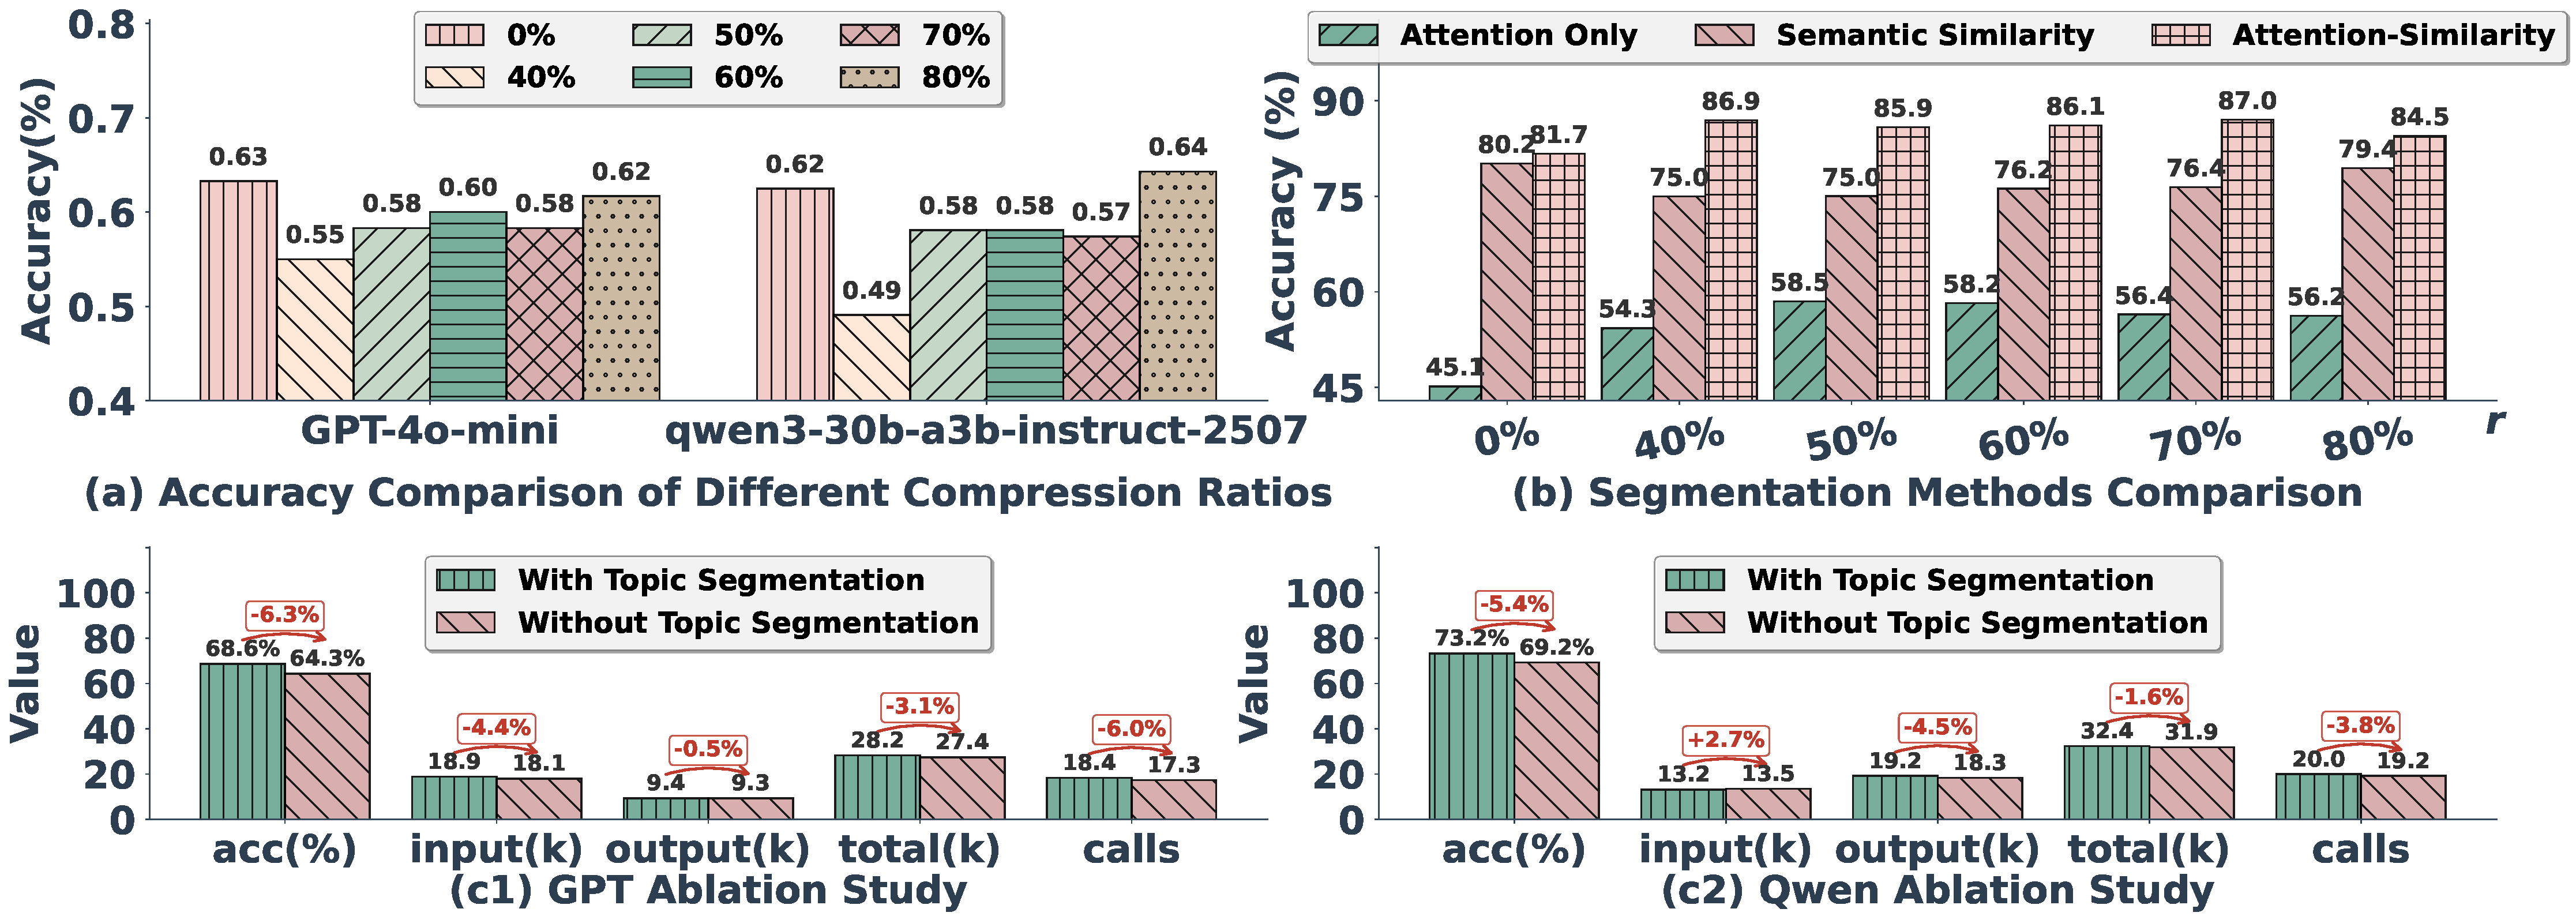
\includegraphics[width=1\textwidth]{figure/figure4.pdf}
    \caption{
    Analysis and Ablation Study of Key Modules. 
    Fig.(a) depicts the QA accuracy when using prompts compressed at different ratios ($r$) as in-contexts to query the LLM directly. 
    Fig.(b) compares the accuracy of different topic segmentation methods under these varying compression ratios. 
    Fig.(c1) and Fig.(c2) present the ablation study for the topic segmentation module, evaluating its impact on both performance and efficiency for the GPT and Qwen models.}
    \label{fig:analysis}
\end{figure*}
\subsection{Analysis of Pre-Compressing Submodule}
\noindent \textbf{Performance and Overhead.}
LightMem uses an additional model~\citep{pan2024llmlingua,xia2025tokenskip} for pre-compression. 
We evaluate its performance by randomly sampling 1/5 of \textsc{LongMemEval} and compressing it at ratios shown in Figure~\ref{fig:analysis}(a), then prompting LLMs for in-context QA. 
When compression ratio $r$ ranges from 50\%--80\%, compressed and uncompressed performance are comparable, demonstrating LLMs can effectively understand compressed content and validating LightMem's approach. 
The submodule is highly efficient, consuming under 2GB of GPU memory with negligible impact on overall runtime.

\noindent \textbf{Impact of $r$ on Performance.}
As shown in Tables~\ref{tab:r_th} and ~\ref{tab:lightmem_comparison}, The optimal $r$ for ACC is dependent on the STM buffer threshold $th$. 
For smaller thresholds ($th \in \{0, 256\}$), an $r$ of 0.6 achieves the highest ACC. 
In contrast, for larger thresholds ($th \in \{512, 1024\}$), a higher retention rate of $r=0.7$ performs best. 
This suggests greater buffer capacity enables effective use of richer, less-compressed information, leveraging LLMs' advanced long-context processing to mitigate the ``lost in the middle'' phenomenon.
On average, the optimal $r$ for ACC is 0.6, reflecting a trade-off between information compression rate and the quantity of information in the STM buffer.
In terms of efficiency, a lower $r$ generally leads to higher efficiency, as it triggers the buffer threshold less frequently under the same $th$, resulting in fewer API calls and lower token consumption.

\subsection{Analysis of Topic Segmentation Submodule}
\noindent \textbf{Segmentation Accuracy.}
To validate the accuracy of our proposed hybrid topic segmentation method, we compare it with segmentation using only a single granularity: attention-only-based and similarity-only-based segmentation. 
Since the construction process of the \textsc{LongMemEval} indicates that different sessions naturally serve as topic boundaries, we directly use them as ground-truth labels. 
The final accuracy is calculated as the number of correctly identified segmentation points divided by the total number of labels. 
The results in Figure~\ref{fig:analysis}(b) validate the effectiveness of our method: it achieves higher accuracy than both individual segmentation methods across all compression ratios, with an absolute accuracy exceeding 80\%.

\noindent \textbf{Ablation Study.}
As shown in Figure~\ref{fig:analysis}(c), removing the topic segmentation submodule slightly improves efficiency but significantly harms accuracy, causing a 6.3\% drop for GPT and 5.4\% for Qwen. 
This indicates that the submodule effectively enables models to perceive semantic units in the input, facilitating subsequent memory unit generation. 

\subsection{Analysis of the STM Threshold's Impact}

As illustrated in the Figure~\ref{fig:lightmem_radar}, the STM buffer threshold ($th$) has a distinct but significant impact on both efficiency and performance metrics.
A consistent trend is: as $th$ increases, there is a marked improvement in efficiency.
In contrast, the effect on QA accuracy is non-monotonic. 
The optimal threshold for accuracy varies depending on the model and the compression ratio ($r$), indicating that a larger buffer does not always yield better performance. 
This highlights a crucial trade-off: 
while a larger STM threshold is consistently better for reducing computational cost, the ideal setting for maximizing task accuracy requires careful tuning.

\subsection{Analysis of Sleep-Time Update}
\label{sec:case_study}
\noindent \textbf{Why Soft Updates Work.}
A primary challenge in designing memory systems is handling updates. 
While powerful, LLMs can be unreliable when tasked with complex real-time update operations. 
For instance, when presented with two related but not contradictory pieces of information, an LLM might incorrectly interpret them as a conflict and delete the older memory entry, leading to irreversible information loss. 
Instead, the optimal operations might be to merge the information or simply add the new entry. 
In contrast, \textbf{LightMem} performs only incremental additions through soft updates during test time, which preserves global information and complete semantics.
\begin{tcolorbox}[
    title=\textbf{Case Study: Memory Update Mechanism Comparison},
    colback=gray!5,
    colframe=black!60,
    fonttitle=\bfseries,
]
\small
\textbf{History1:} \verb|{'Monday, 2 PM': User is planning a trip to Tokyo.}|

\textbf{History2:} \verb|{'Monday, 4 PM': User asks about trains to Kyoto.}|

\noindent
\begin{minipage}[t]{0.49\linewidth}
    \textcolor{red!70!black}{\textbf{Hard Update:}} Overwrites memory
    \\ \texttt{-> "User plans Kyoto trip"}
    \\ \textcolor{red!60}{\faExclamationTriangle\, Tokyo context lost}
\end{minipage}
\hfill
\begin{minipage}[t]{0.49\linewidth}
    \textcolor{green!60!black}{\textbf{LightMem Soft Update:}} Appends info
    \\ \texttt{-> "Tokyo trip + Kyoto inquiry"}  
    \\ \textcolor{green!60}{\faCheckCircle\, Full context preserved}
\end{minipage}
\end{tcolorbox}

% \noindent \textbf{The advantages of offline parallel updates.}
% Table~\ref{tab:lightmem_comparison}  demonstrates the efficiency of our offline update strategy. 
% The data indicates that memory consolidation is not a constant, high-frequency process; only a modest number of update consolidations ($U_{cnt}$) are typically triggered. 
% Moreover, the memory state remains stable, with total entries ($E_{bld}$ vs. 
% $E_{par}$) changing minimally after parallel updates. This signifies that LightMem largely preserves existing memory while efficiently merging relevant information offline. 
% Critically, the $C_{ser}$ column reveals that a conventional online, serial update process would significantly increase latency, by \textbf{5x for GPT} and \textbf{8x for Qwen}. 
% Decoupling consolidation from real-time inference thus allows LightMem to maintain a highly responsive experience, which is crucial for interactive agents.
% \begin{table}[htbp]
\centering
\small
\caption{Sensitivity of memory pipeline. 
$r$: compression ratio; $th$: STM buffer threshold; 
$E_{bld}$: entries after memory build; 
$U_{cnt}$: update count; 
$E_{par}$: entries after parallel updates; 
$C_{ser}$: cost if updates are executed serially (vs.\ parallel).}
\vspace{1ex}
\label{tab:mem-abbrev}
\begin{tabular}{@{}l c c r r r r@{}}
\toprule
Model & $r$ & $th$ & $E_{bld}$ & $U_{cnt}$ & $E_{par}$ & $C_{ser}$ \\
\midrule
\multirow{3}{*}{\textbf{GPT}}
 & 0.5 & 256  & --     & --     & --     & 5x \\
 & 0.6 & 256  & --     & --     & --     & 5x\\
 & 0.7 & 512  & --     & --     & --     & 5x \\
\cmidrule(lr){1-7}
\multirow{3}{*}{\textbf{Qwen}}
 & 0.4 & 768  & 594.36 & 178.40 & 550.09 & 8x \\
 & 0.6 & 768  & 541.99 & 152.93 & 527.23 & 8x \\
 & 0.8 & 1024 & --     & --     & --     & 8x \\
\bottomrule
\end{tabular}
\end{table}
